\documentclass[conference]{IEEEtran}
\IEEEoverridecommandlockouts
% The preceding line is only needed to identify funding in the first footnote. If that is unneeded, please comment it out.
\usepackage{cite}
\usepackage{amsmath,amssymb,amsfonts}
\usepackage{algorithmic}
\usepackage{url}
\usepackage{graphicx}
\usepackage{textcomp}
\usepackage{xcolor}
\usepackage{listings}
\usepackage{tikz}
\lstset{
  basicstyle=\ttfamily\small,
  breaklines=true,
  breakatwhitespace=true,
  columns=fullflexible,
  keepspaces=true,
  frame=single,
  numbers=none,
  keywordstyle=\color{blue},
  commentstyle=\color{gray},
  language=, % <- no language syntax highlighting to prevent overflow issues
}
\def\BibTeX{{\rm B\kern-.05em{\sc i\kern-.025em b}\kern-.08em
    T\kern-.1667em\lower.7ex\hbox{E}\kern-.125emX}}
\begin{document}
\title{Formally Verifying Voter Security Properties in DAO Smart Contracts}

\author{
    \makebox[\textwidth][c]{%
        \begin{minipage}{0.45\textwidth}
            \centering
            \textbf{Anish Toomu} \\
            \textit{Department of Computer Science} \\
            \textit{University of North Carolina at Chapel Hill} \\
            Chapel Hill, North Carolina, USA
        \end{minipage}
        \hfill
        \begin{minipage}{0.45\textwidth}
            \centering
            \textbf{Aidan Maguire} \\
            \textit{Department of Computer Science} \\
            \textit{University of North Carolina at Chapel Hill} \\
            Chapel Hill, North Carolina, USA
        \end{minipage}
    }\\[1.5em]

    \makebox[\textwidth][c]{%
        \begin{minipage}{0.6\textwidth}
            \centering
            \textbf{Jeffrey Zhang} \\
            \textit{Department of Computer Science} \\
            \textit{University of North Carolina at Chapel Hill} \\
            Chapel Hill, North Carolina, USA
        \end{minipage}
    }
}

\maketitle



\section{Abstract}
To be written


\section{Introduction}
This project aims to make use of two existing security tools to define and verify security properties for voting methods across a suite of Ethereum blockchain programs. Many Ethereum blockchain programs take the form of a DAO, or Decentralized Autonomous Organization, wherein users holding tokens that verify them as members of the organization can spend those tokens to vote on decision-making for the DAO as a whole. There are several types of vulnerabilities that have been identified in these types of contracts, but for this paper we will be looking at vulnerabilities surrounding the vote system that allow attackers to exploit the democratic principles behind DAOs.

Our proposal intends to formally verify a suite of the most used DAO contracts to confirm that they are secure. We will require the use of Scribble, a specification language that allows us to define security properties for DAO contracts as annotations within the contracts themselves. We will then use Mythril, a security-analysis tool, to verify each of our newly defined security properties for our suite of popular contracts. If successful, we will increase the confidence in these widely-used contracts. Possible challenges include the properties not being entirely specifiable in Scribble's specification language, and some contracts being too complex to analyze with Mythril due to state explosion.

\section{State of the Art}

DAOs are a type of smart contract that define the rules and structure of a organization. In more general terms, DAOs represent decentralized communities that can allocate resources without centralized leadership. While there exist tools for various methods of verifying and bug-finding in smart contracts including static analysis[1], model checking[2], and symbolic execution[3], they haven’t been narrowed down to focus on DAOs, and the specific exploits that come with their voting systems, a key, shared property across DAOs and a critical part of their operations. We have chosen to use an existing symbolic execution-based tool, Mythril[4], along with Scribble[5], a specification language for properties in this work. 


\section{Background}
To understand our proposed enhancements to Mythril, we must first grasp the fundamental concepts of the blockchain, the Ethereum blockchain and its innovative smart contracts, and finally DAOs, a subset of smart contracts with common functionalities.

\subsection{Blockchain}
A blockchain serves as a ledger of transactions that is transparent, decentralized, and secure. Each block in the chain contains information about transactions allowing anyone to inspect them at any time. Additionally, each block contains a cryptographic hash of the previous block in the chain. This chain means that in the event of a block being tampered with by an attacker, all of the altered blocks' successors would also be changed. The consensus needed to accept a chain also provides further security. If the majority of the computational power on the network is controlled by honest parties then the honest chain will be accepted. An attacker seeking to change a block would need to alter the block, redo all the proof-of-work computation for it and its successor blocks, and then catch up to the honest chain to be accepted. This proves to be computationally infeasible[6].

\subsection{Ethereum and Smart Contracts}
Ethereum, as proposed by Vitalik Buterin in 2014, seeks to provide an alternative to Bitcoin with a focus on the development of decentralized applications. This is achieved through a blockchain that contains a built-in Turing-complete language[7]. This language allows users to write smart contracts that are stored on the blockchain. Smart contracts are a type of account, they have a balance and can be interacted with through transactions. They differ from users’ externally owned accounts in their method of control. Where externally owned accounts are controlled by user decisions, smart contracts are programs that run on the blockchain according to their code. Users or other smart contracts interact with smart contracts by sending a transaction that executes the functions defined by the contract’s code. Smart contracts automatically execute when their conditions are met, are universally visible, and are unable to be changed once uploaded[8]. In this way smart contracts provide a trustworthy, automated way to enforce agreements, reducing the need for third-party enforcement, minimizing exceptions, and lowering the risk of fraud[9].

\subsection{Decentralized Autonomous Organizations}
Decentralized Autonomous Organizations (DAOs) use the blockchain and smart contracts as a way to govern and operate an organization without a central authority. DAOs allow participants to vote on proposed policy changes, actions taken by the organization, and any number of other decisions. These rules are automatically enforced by smart contracts. The first notable DAO, “The DAO” was formed on the Ethereum blockchain in 2016 as a venture capital fund. Users could exchange ether for tokens that gave holders voting power in The DAO proportional to the amount of tokens owned[10]. The organization managed to crowdfund \$168M worth of ether representing one of the largest projects on the Ethereum blockchain. The project is now synonymous with a programming vulnerability in the organization's smart contract that allowed an attacker to siphon off \$50M from The DAO’s[11] gathered funds. This resulted in the controversial hard fork of the Ethereum blockchain and the shuttering of the organization. This example highlights the critical nature of DAO smart contract security as they manage large amounts of currency and interact with a large number of users. Today, a great variety of DAOs exist on Ethereum ranging from communities of creators to venture capital groups[12].

\section{Threat Model}
DAO contract voting vulnerabilities refers to a class of vulnerabilities where an attacker exploits the contract voting mechanism to vote twice with the same tokens, remove other people's votes, vote on a proposal and immediately put it into effect without giving other token holders a chance to vote themselves, or other similar exploits that undermine the decentralized democratic goals of DAO contracts. In our analysis, we assume that attackers have complete visibility of the contract code, and the ability to deploy their own contracts to the blockchain that interface with DAO contracts[13]; however, we are assuming that attackers cannot launch larger Ethereum network attacks such as network congestion or miner manipulation that would require greater coordination and resources. We consider nonvoting-related attacks such as integer overflow, reentrancy, and gas DoS attacks as out of scope for this paper. 

\section{Design}

\subsection{A Formal Model of DAO Smart Contracts}
There is not a prescriptive structure that smart contracts must conform to in order to be considered DAOs, but there are some functionalities that are common to all implementations. All DAOs have a voting function in their contract that allows members to vote on proposals made by other members. We represent the general form of this voting function as a finite state machine related to a given proposal $p \in P$, the set of all proposals in the DAO contract. 
We define the FSM as follows:
\begin{center}
$M = (Q, \Sigma, \delta, q_0, F, u, p, v)$
\end{center}

With $Q$ being the set of voting function states, $\Sigma$ being the set of events triggering changes in state, $\delta$ being the transition function mapping $Q\times\Sigma$, $q_0$ being the initial state, $F$ being the set of terminal states, $u$ being the user that is calling the DAO voting function (either manually or through another smart contract themselves), $p$ is the specific proposal being voted on, and $v$ is the intended vote of the user. All users $u$ have a unique DAO token balance $u_{balance}$ that is tracked by the contract. Additionally, we define $p_{user}$ as a function mapping of $P\times U$: for any given proposal and user, $p_{user}$ holds the current vote of that user. Given this function, we can also reason about a total vote count for each proposal defined as $p_{votes}$ as well as separate counts for each type of vote. For our model, we will only deal with two possible voting decisions, $p_{yes}$ and $p_{no}$, though actual implementations may allow DAO members more variation with the way they vote.

We define the set of states $Q$ as follows:
\begin{figure}[h]
\caption{\textbf{The set $Q$}}
\begin{center}
\begin{tabular}{|c|c|}
\hline
State & Description\\
\hline
$q_0$ & Initial state. $u, v = null$\\
\hline
$q_1$ & $u, v$ are set based on vote request\\
\hline
$q_2$ & $p_{u} = null, u_{balance} > 0$\\
\hline
$Y$ & $p_{yes} += 1$ \\
\hline
$N$ & $p_{no} += 1$\\
\hline
$R$ & $u = null$\\
\hline
$F$ & Proposal voting period ends\\
\hline
\end{tabular}
\end{center}
\end{figure}

And define the set of events $Sigma$ as follows:
\begin{figure}[h]
\caption{\textbf{The set $\Sigma$}}
\begin{center}
\begin{tabular}{|c|c|}
\hline
Event & Description\\
\hline
Function called & Member makes request to contract\\
\hline
Vote validated & Vote request validated (explained below)\\
\hline
Vote yes & Member votes in favor \\
\hline
Vote no & Member votes against\\
\hline
Vote rejected & Vote request is invalid (explained below)\\
\hline
End & End transaction with user and return to initial state\\
\hline
Voting ends & Voting window for the proposal window closes\\
\hline
\end{tabular}
\end{center}
\end{figure}

And finally provide a diagram of the finite state machine for the transition function (Figure 3). Terminating states are indicated with double rings.
\begin{figure}[h]
\begin{center}
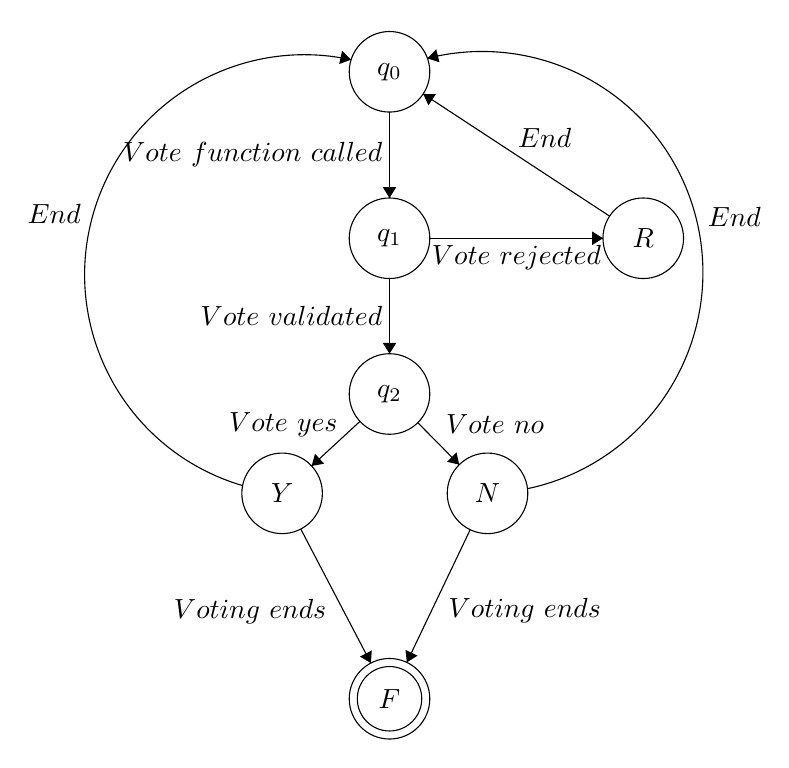
\begin{tikzpicture}[scale=0.1705]
\tikzstyle{every node}+=[inner sep=0pt]
\draw [black] (36.9,-9.6) circle (3);
\draw (36.9,-9.6) node {$q_0$};
\draw [black] (36.9,-22) circle (3);
\draw (36.9,-22) node {$q_1$};
\draw [black] (36.9,-33.6) circle (3);
\draw (36.9,-33.6) node {$q_2$};
\draw [black] (55.8,-22) circle (3);
\draw (55.8,-22) node {$R$};
\draw [black] (44.2,-41) circle (3);
\draw (44.2,-41) node {$N$};
\draw [black] (28.9,-41) circle (3);
\draw (28.9,-41) node {$Y$};
\draw [black] (36.9,-56.3) circle (3);
\draw (36.9,-56.3) node {$F$};
\draw [black] (36.9,-56.3) circle (2.4);
\draw [black] (36.9,-12.6) -- (36.9,-19);
\fill [black] (36.9,-19) -- (37.4,-18.2) -- (36.4,-18.2);
\draw (36.4,-15.8) node [left] {$Vote\mbox{ }function\mbox{ }called$};
\draw [black] (36.9,-25) -- (36.9,-30.6);
\fill [black] (36.9,-30.6) -- (37.4,-29.8) -- (36.4,-29.8);
\draw (36.4,-27.8) node [left] {$Vote\mbox{ }validated$};
\draw [black] (39.9,-22) -- (52.8,-22);
\fill [black] (52.8,-22) -- (52,-21.5) -- (52,-22.5);
\draw (46.35,-22.5) node [below] {$Vote\mbox{ }rejected$};
\draw [black] (39.01,-35.74) -- (42.09,-38.86);
\fill [black] (42.09,-38.86) -- (41.89,-37.94) -- (41.18,-38.65);
\draw (41.08,-35.83) node [right] {$Vote\mbox{ }no$};
\draw [black] (34.7,-35.64) -- (31.1,-38.96);
\fill [black] (31.1,-38.96) -- (32.03,-38.79) -- (31.35,-38.05);
\draw (28.99,-36.81) node [above] {$Vote\mbox{ }yes$};
\draw [black] (53.29,-20.35) -- (39.41,-11.25);
\fill [black] (39.41,-11.25) -- (39.8,-12.1) -- (40.35,-11.27);
\draw (48.46,-15.3) node [above] {$End$};
\draw [black] (25.96,-40.423) arc (-106.3473:-282.23982:16.379);
\fill [black] (34.04,-8.7) -- (33.37,-8.04) -- (33.15,-9.02);
\draw (13.94,-20.19) node [left] {$End$};
\draw [black] (39.724,-8.599) arc (104.2931:-78.11737:16.458);
\fill [black] (39.72,-8.6) -- (40.62,-8.89) -- (40.38,-7.92);
\draw (60.57,-20.41) node [right] {$End$};
\draw [black] (30.29,-43.66) -- (35.51,-53.64);
\fill [black] (35.51,-53.64) -- (35.58,-52.7) -- (34.7,-53.16);
\draw (32.22,-49.8) node [left] {$Voting\mbox{ }ends$};
\draw [black] (42.91,-43.71) -- (38.19,-53.59);
\fill [black] (38.19,-53.59) -- (38.99,-53.09) -- (38.09,-52.66);
\draw (41.26,-49.71) node [right] {$Voting\mbox{ }ends$};
\end{tikzpicture}
\end{center}
\caption{DAO Voting contract Finite State Machine}
\end{figure}

As stated above, this model represents the possible state space for the voting function of a given proposal. 

This formal model provides the foundation for our conception of DAO smart contracts. As our goal is to verify the voting functionality of DAOs, it follows that we are focused primarily on the \textit{Vote Validated} event transition, and this is where most of our verification efforts will take place. Defining what it means for a vote to be validated will lead us to introduce our security properties.

\subsection{Security Properties for Secure DAO Voting}
We describe three basic properties for a secure DAO voting system:
\begin{enumerate}
    \item Singular Vote: A single member of the DAO should not be able to vote more than once, or have their vote count for more than one vote.
    \item Vote Authorization: Anyone can make a vote request using the contract, but only DAO members (holders of the particular DAO token) should be able to vote.
    \item Quorum Threshold: For a DAO proposal to be finalized, a minimum portion of the total eligible voters need to have voted. This prevents proposals from being enacted that only got a single yes vote, for example.
\end{enumerate}

We formalize these properties according to the $Vote\mbox{ }Validated$ event.
For the $Vote\mbox{ }Validated$ event to trigger and to go from state $A$ to state $B$:
\begin{center}
$p_{user} = null \land u_{balance} > 0$. 
\end{center}
This ensures that potential voters are authorized members who have not already voted. We also need to define a second property to make sure that the proper behavior occurs when our contract terminates according to the current state of the FSM $q$ and initial state $q_{0}$:
\begin{center}
    $q \in\{Y,N\}\xrightarrow{}p_{user} \neq null \land p_{votes} - p_{votes}^0 = 1$
\end{center}

Where $p_{votes}^0$ is the value of $p_{votes}$ in the initial state of execution $q_0$. This ensures that votes are counted once and only once. 

The final security property, Quorum Threshold, 

\section{Implementation}
\subsection{Workflow}

We started by defining our basic voting security properties in the DAOProperties.spec file. 

\begin{lstlisting}[basicstyle=\ttfamily\small,breaklines=true]
    /// @title DAO Properties Specification
    /// @notice Abstract properties that should hold for any DAO implementation

    /// @property {:msg "Only token holders can vote"} 
    ///     tokenBalances[msg.sender] > 0 || isMember[msg.sender] == true;

    /// @property {:msg "Single vote per address"} 
    ///     proposals[_proposalId].hasVoted[msg.sender] == true;

    /// @property {:msg "Quorum is met before execution"} 
    ///     (proposals[_proposalId].yesVotes + proposals[_proposalId].noVotes) >= 
    ///     (totalTokens * QUORUM_THRESHOLD) / 100 || 
    ///     proposals[_proposalId].numberOfVotes >= minimumQuorum;
\end{lstlisting}


We then manually annotated the target functions in the smart contract code with these properties. When we run Scribble on the annotated contract, it rewrites the Solidity source contract so that every property becomes a run-time assertion. We then feed this instrumented contract to Mythril, which symbolically explores all possible execution paths. If Mythril finds a path that violates one of our annotated conditions, it raises an AssertionFailed event with a corresponding message. 

Before we tried to annotate real world contracts, we built three deliberately flawed “toy” contracts: one for each vulnerability we were focusing on. This allowed us to tune our Scribble annotations on a simple contract with a much faster turnaround than having to wait hours for a complex contract to finish evaluating. 

The first toy contract (Figure 1) omits any check on a caller’s token balance, so non-holders can vote freely. The second (Figure 2) remembers votes in a mapping but never consults that mapping, allowing the same address to vote twice. The third (Figure 3) allows execution as soon as a “yes” majority exists, without verifying that the total number of votes meets the quorum threshold.




\subsection{Toy Examples}

\begin{figure}[h]
\centering
\begin{lstlisting}[basicstyle=\ttfamily\small,breaklines=true]
    // Flawed logic: No token balance check
    
    /// @property {:msg "Only token holders can vote"} 
    ///     tokenBalances[msg.sender] > 0 || isMember[msg.sender] == true;
    
    function vote(uint256 proposalId, bool support) external {
        // Missing token balance check
        Proposal storage p = proposals[proposalId];
        
        if (support) {
            p.yesVotes += 1;
        } else {
            p.noVotes += 1;
        }
        p.numberOfVotes += 1;
    }
\end{lstlisting}
\caption{Authorization property: Only token holders can vote.}
\label{fig:auth_property}
\end{figure}

\begin{figure}[h]
\centering
\begin{lstlisting}[basicstyle=\ttfamily\small,breaklines=true]
    // Flawed logic: No check for previous votes
    
    /// @property {:msg "Single vote per address"} 
    ///     proposals[_proposalId].hasVoted[msg.sender] == true;
    
    function vote(uint256 proposalId, bool support) external {
        require(tokenBalances[msg.sender] > 0, "No tokens");
        Proposal storage p = proposals[proposalId];
        
        // Missing hasVoted check
        if (support) {
            p.yesVotes += 1;
        } else {
            p.noVotes += 1;
        }
        p.numberOfVotes += 1;
    }
\end{lstlisting}
\caption{Single vote property: Each address can only vote once per proposal.}
\label{fig:single_vote_property}
\end{figure}

\begin{figure}[h]
\centering
\begin{lstlisting}[basicstyle=\ttfamily\small,breaklines=true]
    // Flawed logic: No quorum check before execution
    
    /// @property {:msg "Quorum is met before execution"} 
    ///     (proposals[_proposalId].yesVotes + proposals[_proposalId].noVotes) >= 
    ///     (totalTokens * QUORUM_THRESHOLD) / 100 || 
    ///     proposals[_proposalId].numberOfVotes >= minimumQuorum;
    
    function executeProposal(uint256 proposalId) external {
        Proposal storage p = proposals[proposalId];
        
        // Missing quorum check
        if (p.yesVotes > p.noVotes) {
            // Execute proposal
            p.executed = true;
        }
    }
\end{lstlisting}
\caption{Quorum property: Quorum must be met before execution.}
\label{fig:quorum_property}
\end{figure}
\section{Evaluation}
We evaluate 4 DAO smart contracts using the workflow outlined in Section VII. 
\subsection{SimpleDAO} The first contract we examine is SimpleDAO. We create SimpleDAO as a basic DAO with token-weighted voting, quorum-dependent proposal execution, and self-contained code with no external calls. The Mythril symbolic execution analyzes the instrumented Solidity file finding no violation of the voting security properties.
\subsection{FlawedDAO} The second example contract is FlawedDAO. This is a basic DAO contract that violates all of the voting security properties as a demonstration. The Mythril analysis of the contract results in the marking of all three violations.
\subsection{dao-congress} The original specifications were designed for a token-based voting system, which we had to modify to accommodate the membership-based architecture of the Congress DAO implementation. For the authorization property, we replaced the token balance check with a membership verification, ensuring that only registered members (where memberId[msg.sender] != 0) can participate in voting. The single-vote-per-address property was implemented by verifying the state of the voted mapping after each vote transaction. Finally, the quorum requirement was adapted from a percentage-based token threshold to a simple vote count comparison against a minimum quorum value. 

\begin{figure}[h]
\centering
\begin{lstlisting}[basicstyle=\ttfamily\small,breaklines=true]
SWC ID: 110
Severity: Medium
Contract: FlawedDAO
Function name: finalize(uint256)
PC address: 913
Estimated Gas Usage: 16596 - 39024
A user-provided assertion failed.
--------------------
In file: contracts/FlawedDAO.sol:123
__ScribbleUtilsLib__373.AssertionFailed ("004763:0097:000 6: Quorum is met before execution")
--------------------

==== Exception State ====
SWC ID: 110
Severity: Medium
Contract: FlawedDAO
Function name: vote(uint256,bool)
PC address: 1993
Estimated Gas Usage: 13941 - 36039
A user-provided assertion failed.
--------------------
In file: contracts/FlawedDAO.sol:94
__ScribbleUtilsLib__373.AssertionFailed( "003414:0094:000 4: Only token holders can vote")
--------------------
==== Exception State ====
SWC ID: 110
Severity: Medium
Contract: FlawedDAO
Function name: vote(uint256,bool)
PC address: 2157
Estimated Gas Usage: 14962 - 37770
A user-provided assertion failed.
--------------------
In file: contracts/FlawedDAO.sol:98
__ScribbleUtilsLib__373.AssertionFailed ("003637:0090:000 5: Single vote per address")
--------------------
\end{lstlisting}
\caption{Mythril output flagging property violations in \texttt{FlawedDAO}.}
\label{fig:flawed_dao_assertions}
\end{figure}

\subsection{Association} The fourth contract we evaluate is Association CITE. This is an open-source DAO contract developed by the Ethereum Foundation. This contract represents a shareholder-controlled organization in which token holders vote on transactions that send funds to the proposed recipient. This contract is more complex than the previous examples, containing external calls to the \texttt{Token} interface and inheriting from two contracts. Mythril models external calls conservatively, assuming that the called function can result in any return. To accurately model the authorization property correctly, we create a hard-coded \texttt{mockBalanceOf} mapping locally that allows Mythril to reason about \texttt{sharesTokenAddress.balanceOf()} properly. For the quorum property, we add a helper function \texttt{hasQuorum()} to count the proposal's proportion of shares stored in an array of vote objects. This is done because Scribble does not provide functionality to loop and sum over an array.
The greater complexity of the Association contract resulted in a state space explosion; unbounded symbolic execution of the contract led to segmentation faults and run times exceeding an hour. To counteract this, we tested the properties separately with bounded depth and runtime. During these bounded analyses, all three voting security properties held.


\section{Conclusion}
To be written

\section{Who Did What}
\begin{itemize}
    \item Aidan: Contributed to the Introduction, Threat Model, and References
    \item Anish: Contributed to the Approach, Set up repository, dependencies, and starter DAO contract/annotations
    \item Jeffrey: Contributed to the Background, State of the Art, and Evaluation sections
\end{itemize}

\begin{thebibliography}{00}
\bibitem{b1} J. Feist, G. Grieco, and A. Groce, “Slither: A static analysis framework for smart contracts,” 2019, pp. 8–15. Available: \url{https://ieeexplore.ieee.org/abstract/document/8823898?casa_token=SNthQs5W2d0AAAAA:XwX332JMCkj3hw8XZd9nKBxe2bKJZ3v3yUNJ3jPtangZ3L2nISxh_rbY8fBW2zXkaWa0QnqgqVE}
\bibitem{b2} Z. Nehaï, P.-Y. Piriou, and F. Daumas, “Model-checking of smart contracts,” 2018, pp. 980–987. Available: \url{https://ieeexplore.ieee.org/abstract/document/8726806}
\bibitem{b3} J. He, M. Balunović, N. Ambroladze, P. Tsankov, and M. Vechev, “Learning to Fuzz from Symbolic Execution with Application to Smart Contracts,” Proceedings of the 2019 ACM SIGSAC Conference on Computer and Communications Security, pp. 531–548, Nov. 2019, Available: \url{https://dl.acm.org/doi/abs/10.1145/3319535.3363230?casa_token=5cBcZneJt7oAAAAA:sPluGu-gtO_db3qLqHUcylo4ksy4Rx0FBkiEBFom7You4VltkgLyZanIwgg-WHfLDVmrwmU0MbdpGA}
\bibitem{b4} N. Sharma and S. Sharma, “A Survey of Mythril, A Smart Contract Security Analysis Tool for EVM Bytecode,” Indian Journal of Natural Sciences, vol. 12, no. 75, Dec. 2022, Available:
\url{https://www.researchgate.net/profile/Swati-Sharma-171/publication/366391033_A_Survey_of_Mythril_A_Smart_Contract_Security_Analysis_Tool_for_EVM_Bytecode/links/639ecbdc095a6a77743c8073/A-Survey-of-Mythril-A-Smart-Contract-Security-Analysis-Tool-for-EVM-Bytecode.pdf}
\bibitem{b5} ConsenSysDiligence, “GitHub - ConsenSysDiligence/scribble: Scribble instrumentation tool,” GitHub, Apr. 09, 2025. Available:  
\url{ConsenSysDiligence, “GitHub - ConsenSysDiligence/scribble: Scribble instrumentation tool,” GitHub, Apr. 09, 2025. https://github.com/ConsenSysDiligence/scribble/tree/develop (accessed Apr. 10, 2025).}
\bibitem{6} S. Nakamoto, “Bitcoin: a Peer-to-Peer Electronic Cash System,” bitcoin.org, Oct. 2008. Available: 
\url{https://bitcoin.org/bitcoin.pdf}
\bibitem{7} V. Buterin, “Ethereum Whitepaper,” Ethereum, 2014. Available: 
\url{https://ethereum.org/en/whitepaper/}
\bibitem{8} P. Wackerow, “Introduction to smart contracts,” ethereum.org, Sep. 02, 2022. Available: 
\url{https://ethereum.org/en/developers/docs/smart-contracts/}
\bibitem{9} N. Szabo, “Smart Contracts,” www.fon.hum.uva.nl, 1994. 
\url{https://www.fon.hum.uva.nl/rob/Courses/InformationInSpeech/CDROM/Literature/LOTwinterschool2006/szabo.best.vwh.net/smart.contracts.html}
\bibitem{10} C. Jentzsch, “DECENTRALIZED AUTONOMOUS ORGANIZATION TO AUTOMATE GOVERNANCE,” 2016. Available: 
\url{https://lawofthelevel.lexblogplatformthree.com/wp-content/uploads/sites/187/2017/07/WhitePaper-1.pdf}
\bibitem{11} C. Shier et al., “Understanding a Revolutionary and Flawed Grand Experiment in Blockchain: The DAO Attack,” SSRN Electronic Journal, 2017, doi: 
\url{https://doi.org/10.2139/ssrn.3014782.}
\bibitem{12} “List of 41 DAOs (2025),” Alchemy, 2025. Available:
\url{https://www.alchemy.com/dapps/top/daos}
\bibitem{13} K. Nekrasov, “DAO Voting Vulnerabilities,” Mixbytes.io, 2024.
\url{https://mixbytes.io/blog/dao-voting-vulnerabilities}
\bibitem{14} HausDAO, “GitHub - HausDAO/Molochv2.1: Moloch DAO v2 with multi-summoner capabilities, plus register function for metadata.,” GitHub, 2020. Available:
\url{https://github.com/HausDAO/Molochv2.1}
\end{thebibliography}
\end{document}
